%%%%%%%%%%%%%%%%%%%%%%%%%%%%%%%%%%%%%%%%%
% Programming/Coding Assignment
% LaTeX Template
%
% This template has been downloaded from:
% http://www.latextemplates.com
%
% Original author:
% Ted Pavlic (http://www.tedpavlic.com)
%
% Note:
% The \lipsum[#] commands throughout this template generate dummy text
% to fill the template out. These commands should all be removed when 
% writing assignment content.
%
% This template uses a Perl script as an example snippet of code,
% most other languages are also usable. Configure them in the
% "CODE INCLUSION CONFIGURATION" section.
%%%%%%%%%%%%%%%%%%%%%%%%%%%%%%%%%%%%%%%%%

%-------------------------------------------------------------------------
%	PACKAGES AND OTHER DOCUMENT CONFIGURATIONS
%-------------------------------------------------------------------------

\documentclass{article}

\usepackage{fancyhdr} % Required for custom headers
\usepackage{lastpage} % Required to determine the last page for the footer
\usepackage{extramarks} % Required for headers and footers
\usepackage[usenames,dvipsnames]{color} % Required for custom colors
\usepackage{graphicx} % Required to insert images
\usepackage{listings} % Required for insertion of code
\usepackage{courier} % Required for the courier font
\usepackage{hyperref}
\usepackage{amsmath}
\usepackage{mathrsfs}
\usepackage{float}
\usepackage{enumitem}
\usepackage[english]{babel}
\usepackage[utf8]{inputenc}
\usepackage{fontenc}
\usepackage{booktabs}
% Margins
\topmargin=-0.45in
\evensidemargin=0in
\oddsidemargin=0in
\textwidth=6.5in
\textheight=9.0in
\headsep=0.25in

\linespread{1.1} % Line spacing

% Set up the header and footer
\pagestyle{fancy}
\lhead{\hmwkAuthorName} % Top left header
\chead{\hmwkClassShort\ (\hmwkClassInstructor)} % Top center head
%\rhead{\firstxmark} % Top right header
\rhead{\hmwkTitle}
\lfoot{\lastxmark} % Bottom left footer
\cfoot{} % Bottom center footer
% Bottom right footer
\rfoot{Page\ \thepage\ of\ \protect\pageref{LastPage}} 
\renewcommand\headrulewidth{0.4pt} % Size of the header rule
\renewcommand\footrulewidth{0.4pt} % Size of the footer rule

\setlength\parindent{0pt} % Removes all indentation from paragraphs

%--------------------------------------------------------------------------
%	CODE INCLUSION CONFIGURATION
%--------------------------------------------------------------------------
% This is the color used for comments
\definecolor{MyDarkGreen}{rgb}{0.0,0.4,0.0} 
\lstloadlanguages{Perl,Python} % Load Perl syntax for listings,
% for a list of other languages supported see:
%ftp://ftp.tex.ac.uk/tex-archive/macros/latex/contrib/listings/listings.pdf
\lstset{language=Perl, % Use Perl in this example
        frame=single, % Single frame around code
        basicstyle=\small\ttfamily, % Use small true type font
        keywordstyle=[1]\color{Blue}\bf, % Perl functions bold and blue
        keywordstyle=[2]\color{Purple}, % Perl function arguments purple
        % Custom functions underlined and blue
        keywordstyle=[3]\color{Blue}\underbar, 
        identifierstyle=, % Nothing special about identifiers
        % Comments small dark green courier font
        commentstyle=\usefont{T1}{pcr}{m}{sl}\color{MyDarkGreen}\small, 
        stringstyle=\color{Purple}, % Strings are purple
        showstringspaces=false, % Don't put marks in string spaces
        tabsize=5, % 5 spaces per tab
        %
        % Put standard Perl functions not included
        % in the default language here
        morekeywords={rand},
        %
        % Put Perl function parameters here
        morekeywords=[2]{on, off, interp},
        %
        % Put user defined functions here
        morekeywords=[3]{test},
       	%
        % Line continuation (...) like blue comment
        morecomment=[l][\color{Blue}]{...}, 
        numbers=left, % Line numbers on left
        firstnumber=1, % Line numbers start with line 1
        numberstyle=\tiny\color{Blue}, % Line numbers are blue and small
        stepnumber=5 % Line numbers go in steps of 5
}


\lstset{language=Python, % Use Python in this example
        frame=single, % Single frame around code
        basicstyle=\small\ttfamily, % Use small true type font
        keywordstyle=[1]\color{Blue}\bf, % Python functions bold and blue
        keywordstyle=[2]\color{Purple}, % Python function arguments purple
        % Custom functions underlined and blue
        keywordstyle=[3]\color{Blue}\underbar, 
        identifierstyle=, % Nothing special about identifiers
        % Comments small dark green courier font
        commentstyle=\usefont{T1}{pcr}{m}{sl}\color{MyDarkGreen}\small, 
        stringstyle=\color{Purple}, % Strings are purple
        showstringspaces=false, % Don't put marks in string spaces
        tabsize=3, % 5 spaces per tab
        %
        % Put standard Python functions not included in the
        % default language here
        morekeywords={rand},
        %
        % Put Python function parameters here
        morekeywords=[2]{on, off, interp},
        %
        % Put user defined functions here
        morekeywords=[3]{test},
       	%
        % Line continuation (...) like blue comment
        morecomment=[l][\color{Blue}]{...}, 
        numbers=left, % Line numbers on left
        firstnumber=1, % Line numbers start with line 1
        numberstyle=\tiny\color{Blue}, % Line numbers are blue and small
        stepnumber=5 % Line numbers go in steps of 5
}


% Creates a new command to include a perl script, the first
% parameter is the filename of the script (without .pl), the
% second parameter is the caption
\newcommand{\perlscript}[2]{
\begin{itemize}
\item[]\lstinputlisting[caption=#2,label=#1]{#1.pl}
\end{itemize}
}
\newcommand{\pythonscript}[2]{
\begin{itemize}
\item[]\lstinputlisting[caption=#2,label=#1]{#1}
\end{itemize}
}
\newcommand{\tss}{\textsuperscript}
\newcommand{\tsbs}{\textsubscript}

%--------------------------------------------------------------------------
%	DOCUMENT STRUCTURE COMMANDS
%	Skip this unless you know what you're doing
%--------------------------------------------------------------------------

% Header and footer for when a page split occurs within a
% problem environment
\newcommand{\enterProblemHeader}[1]{
\nobreak\extramarks{#1}{#1 continued on next page\ldots}\nobreak
\nobreak\extramarks{#1 (continued)}{#1 continued on next page\ldots}\nobreak
}

% Header and footer for when a page split occurs between problem
% environments
\newcommand{\exitProblemHeader}[1]{
\nobreak\extramarks{#1 (continued)}{#1 continued on next page\ldots}\nobreak
\nobreak\extramarks{#1}{}\nobreak
}

\setcounter{secnumdepth}{0} % Removes default section numbers
% Creates a counter to keep track of the number of problems
\newcounter{homeworkProblemCounter} 

\newcommand{\homeworkProblemName}{}
\newenvironment{homeworkProblem}[1][Problem \arabic{homeworkProblemCounter}]{ % Makes a new environment called homeworkProblem which takes
   % 1 argument (custom name) but the default is "Problem #"
  % Increase counter for number of problems
  \stepcounter{homeworkProblemCounter}
  % Assign \homeworkProblemName the name of the problem
  \renewcommand{\homeworkProblemName}{#1}
  % Make a section in the document with the custom problem count
  \section{\homeworkProblemName}
  % Header and footer within the environment  
  \enterProblemHeader{\homeworkProblemName} 
}{
  % Header and footer after the environment
  \exitProblemHeader{\homeworkProblemName}
}
% Defines the problem answer command with the content as the only argument
 % Makes the box around the problem answer and puts the content inside
\newcommand{\problemAnswer}[1]{ 
\noindent\framebox[\columnwidth][c]{\begin{minipage}{0.98\columnwidth}#1\end{minipage}}
}

\newcommand{\homeworkSectionName}{}
\newenvironment{homeworkSection}[1]{ % New environment for sections within homework problems, takes 1 argument - the name of the section
\renewcommand{\homeworkSectionName}{#1} % Assign \homeworkSectionName to the name of the section from the environment argument
\subsection{\homeworkSectionName} % Make a subsection with the custom name of the subsection
\enterProblemHeader{\homeworkProblemName\ [\homeworkSectionName]} % Header and footer within the environment
}{
\enterProblemHeader{\homeworkProblemName} % Header and footer after the environment
}

%--------------------------------------------------------------------------
%	NAME AND CLASS SECTION
%--------------------------------------------------------------------------
\newcommand{\hmwkTitle}{Homework\ 2} % Assignment title
\newcommand{\hmwkDueDate}{Wednesday,\ October\ 19,\ 2016} % Due date
\newcommand{\hmwkClass}{NUEN 647\\ Uncertainty Quantification for Nuclear Engineering} % Course/class
\newcommand{\hmwkClassTime}{Tu/Th 11:10am} % Class/lecture time
\newcommand{\hmwkClassInstructor}{Dr. McClarren} % Teacher/lecturer
\newcommand{\hmwkAuthorName}{Paul Mendoza} % Your name
\newcommand{\hmwkClassShort}{NUEN 647 UQ for Nuclear Engineering}
%--------------------------------------------------------------------------
%	TITLE PAGE
%--------------------------------------------------------------------------

\title{
\vspace{2in}
\textmd{\textbf{\hmwkClass\ \hmwkTitle}}\\
\normalsize\vspace{0.1in}\small{Due\ on\ \hmwkDueDate}\\
\vspace{0.1in}\large{\textit{\hmwkClassInstructor}}
\vspace{3in}
}

\author{\textbf{\hmwkAuthorName}}
\date{} % Insert date here if you want it to appear below your name

%--------------------------------------------------------------------------

\begin{document}

\maketitle

%--------------------------------------------------------------------------
%	TABLE OF CONTENTS
%--------------------------------------------------------------------------

%\setcounter{tocdepth}{1} % Uncomment this line if you don't want subsections listed in the ToC

\newpage
\tableofcontents
\newpage

%--------------------------------------------------------------------------
%	PROBLEM 1
%--------------------------------------------------------------------------

% To have just one problem per page, simply put a \clearpage after each problem

\begin{homeworkProblem}
  Consider a covariance function between points in 2-D space:
  \begin{equation*}
    k(x_1,y_1,x_2,y_2)=exp[-|x_1-x_2|-|y_1-y_2|]
  \end{equation*}
  Generate 4 realizations of a Gaussian random process with zero mean,
  $\mu(x,y)=0$, and this covariance function defined on the unit square,
  $x,y\in [0,1]$. For the realizations, evaluate the process at 50
  equally space points in each direction. Plot the realizations. 
\end{homeworkProblem}

\clearpage

%--------------------------------------------------------------------------
%	PROBLEM 2
%--------------------------------------------------------------------------

\begin{homeworkProblem}
  Assume you have 100 samples of a pair of random variables
  $(X_1,X_2)$ that have a positive correlation, call this set
  of pairs, $\mathbf{A_1}$. You then draw another 100 samples and
  call this set $\mathbf{A_2}$. The Pearson correlation between
  $(X_1,X_2)$ in $\mathbf{A_1}$ is positive and hte Pearson correlation
  between $(X_1,X_2)$ in $\mathbf{A_2}$ is negative. What can you
  say about the Pearson correlation for all 200 samples?
  \vspace{5mm}
  
  \problemAnswer{
    \vspace{3mm}
    A normalized measure of the relation between two random variables,
    is the Pearson correlation coefficient, $\rho$. Oftentimes,
    this is simply called the correlation coefficient or correlation.
    \begin{equation*}
      \rho(X_1,X_2)=\frac{E[X_1X_2]-E[X_1]E[X_2]}
          {\sigma_{X1}\sigma_{X2}}
    \end{equation*}
    The expectation value for a series of realizations is defined:
    \begin{equation*}
      E[g(x)]\approx\frac{1}{N}\sum_{i=1}^{N}g(x_i)
    \end{equation*}
    \\~\\
    For the first 100 values:
    \begin{align*}
      \rho_1&=\frac{\frac{1}{100}\sum_{i=1}^{100}X_{1,i}X_{2,i}-
      \frac{1}{10000}\sum_{i=1}^{100}X_{1,i}\sum_{i=1}^{100}X_{2,i}}
          {\sigma_{X1,A1}\sigma_{X2,A1}}\\
          100\sigma_{X1,A1}\sigma_{X2,A1}\rho_1&=
          \sum_{i=1}^{100}X_{1,i}X_{2,i}-
          \frac{1}{100}\sum_{i=1}^{100}X_{1,i}\sum_{i=1}^{100}X_{2,i}\\
          100\sigma_{X1,A1}\sigma_{X2,A1}\rho_1+
          \frac{1}{100}\sum_{i=1}^{100}X_{1,i}\sum_{i=1}^{100}X_{2,i}
          &=
          \sum_{i=1}^{100}X_{1,i}X_{2,i}
    \end{align*}
    Similarly for the second 100 values:
    \begin{equation*}
      \sum_{i=101}^{200}X_{1,i}X_{2,i}=
      100\sigma_{X1,A2}\sigma_{X2,A2}\rho_2+
      \frac{1}{100}\sum_{i=101}^{200}X_{1,i}\sum_{i=101}^{200}X_{2,i}
    \end{equation*}
    The Pearson coefficient for all 200 values:
    \begin{align*}
      \rho_3&=\frac{\frac{1}{200}\sum_{i=1}^{200}X_{1,i}X_{2,i}-
      \frac{1}{40000}\sum_{i=1}^{200}X_{1,i}\sum_{i=1}^{200}X_{2,i}}
          {\sigma_{X1,A3}\sigma_{X2,A3}}\\
          200\sigma_{X1,A3}\sigma_{X2,A3}\rho_3&=
          \sum_{i=1}^{200}X_{1,i}X_{2,i}-
          \frac{1}{200}\sum_{i=1}^{200}X_{1,i}\sum_{i=1}^{200}X_{2,i}\\
          200\sigma_{X1,A3}\sigma_{X2,A3}\rho_3+
          \frac{1}{200}\sum_{i=1}^{200}X_{1,i}\sum_{i=1}^{200}X_{2,i}
          &=
          \sum_{i=1}^{200}X_{1,i}X_{2,i}
    \end{align*}
    If we plug in the Pearson for the first 100 and second 100 for the
    right side of the equation,
  }
  \clearpage
    \begin{align*}
          200\sigma_{X1,A3}\sigma_{X2,A3}\rho_3&+
          \frac{1}{200}\sum_{i=1}^{200}X_{1,i}\sum_{i=1}^{200}X_{2,i}\\
          &=\\
          100(\sigma_{X1A1}\sigma_{X2A1}\rho_1
          &+\sigma_{X1A2}\sigma_{X2A2}\rho_2)+
          \frac{1}{100}\left(\sum_{i=1}^{100}x_{1,i}\sum_{i=1}^{100}x_{2,i}
          +\sum_{i=101}^{200}x_{1,i}\sum_{i=101}^{200}x_{2,i}\right)
    \end{align*}
    Grouping and setting:
    \begin{center}
    $\sum_{i=1}^{100}x_{1,i}=X_{1,1}$\\~\\
    $\sum_{i=1}^{100}x_{2,i}=X_{2,1}$\\~\\
    $\sum_{i=101}^{200}x_{1,i}=X_{1,2}$\\~\\
    $\sum_{i=101}^{200}x_{2,i}=X_{2,2}$\\~\\
    $\sum_{i=1}^{200}x_{1,i}=X_{1,3}$ \\~\\
    $\sum_{i=1}^{200}x_{2,i}=X_{2,3}$
    \end{center}
    \begin{align*}
      200\sigma_{X1,A3}\sigma_{X2,A3}\rho_3-
      100(\sigma_{X1A1}\sigma_{X2A1}\rho_1
      +\sigma_{X1A2}\sigma_{X2A2}\rho_2)
      =
      \frac{1}{100}\left(X_{1,1}X_{2,1}
      +X_{1,2}X_{2,2}\right)-
      \frac{1}{200}X_{1,3}X_{2,3}
    \end{align*}
    Setting:
    \begin{center}
      $\sigma_{X1A1}=\frac{1}{100}\sum_{i=1}^{100}
      (x_{1,i}^2-\mu_{X_{11}}^2)=\frac{1}{100}\sigma_{X1A1}'$\\~\\
      $\sigma_{X2A1}=\frac{1}{100}\sum_{i=1}^{100}
      (x_{2,i}^2-\mu_{X_{21}}^2)=\frac{1}{100}\sigma_{X2A1}'$\\~\\
      $\sigma_{X1A2}=\frac{1}{100}\sum_{i=101}^{200}
      (x_{1,i}^2-\mu_{X_{12}}^2)=\frac{1}{100}\sigma_{X1A2}'$\\~\\
      $\sigma_{X2A2}=\frac{1}{100}\sum_{i=101}^{200}
      (x_{2,i}^2-\mu_{X_{22}}^2)=\frac{1}{100}\sigma_{X2A2}'$\\~\\
      $\sigma_{X1A3}=\frac{1}{200}\sum_{i=1}^{200}
      (x_{1,i}^2-\mu_{X_{13}}^2)=\frac{1}{200}\sigma_{X1A3}'$\\~\\
      $\sigma_{X2A3}=\frac{1}{200}\sum_{i=1}^{200}
      (x_{2,i}^2-\mu_{X_{23}}^2)=\frac{1}{200}\sigma_{X2A3}'$\\~\\
    \end{center}
    Where $A3$ and $\rho_3$ are for the series added to 200. Plugging
    these in, and multiplying both sides of the equation by 200.
    \begin{align*}
      \sigma_{X1,A3}'\sigma_{X2,A3}'\rho_3-
      2(\sigma_{X1A1}'\sigma_{X2A1}'\rho_1
      +\sigma_{X1A2}'\sigma_{X2A2}'\rho_2)
      =
      2\left(X_{1,1}X_{2,1}
      +X_{1,2}X_{2,2}\right)-
      X_{1,3}X_{2,3}
    \end{align*}
    Note: $X_{1,3}=X_{1,1}+X_{2,1}$ and $X_{2,3}=X_{2,1}+X_{2,2}$
    and that the right side of the equation simplifies to:
    $(X_{1,1}-X_{1,2})(X_{2,1}-X_{2,2})$. Then $\rho_3$ is:
    \begin{align*}
      \rho_3
      =\frac{(X_{1,1}-X_{1,2})(X_{2,1}-X_{2,2})+
      2(\sigma_{X1A1}'\sigma_{X2A1}'\rho_1
      +\sigma_{X1A2}'\sigma_{X2A2}'\rho_2)}
      {\sigma_{X1,A3}'\sigma_{X2,A3}'}
    \end{align*}
    Assuming that:
    \begin{align*}
      \frac{(X_{1,1}-X_{1,2})(X_{2,1}-X_{2,2})}
           {\sigma_{X1,A3}'\sigma_{X2,A3}'}\approx0\\
    \end{align*}
    and
    \begin{align*}
      \sigma_{X1,A3}'\sigma_{X2,A3}'&\approx
      4\sigma_{X1A1}'\sigma_{X2A1}'\\ or &\approx
      4\sigma_{X1A2}'\sigma_{X2A2}'
    \end{align*}
    The above would simplify to:
    \begin{align*}
      \rho_3\approx\frac{\rho_1+\rho_2}{2}
    \end{align*}
    Meaning, $\rho_3$ will usually be inside the interval
    $\rho_2<\rho_3<\rho_1$, I was curious, and wrote a script,
    to check to see if it would ever be outside. There could
    be an error with my script, but I found with the below script
    that a small percentage (less than 1\% of the time),
    it would be outside the above interval. I also made a histogram
    plot...because I like wasting time.

    \pythonscript{Problem2/Calculations}{Script for Problem}
    \begin{figure}[H]
      \begin{center}
        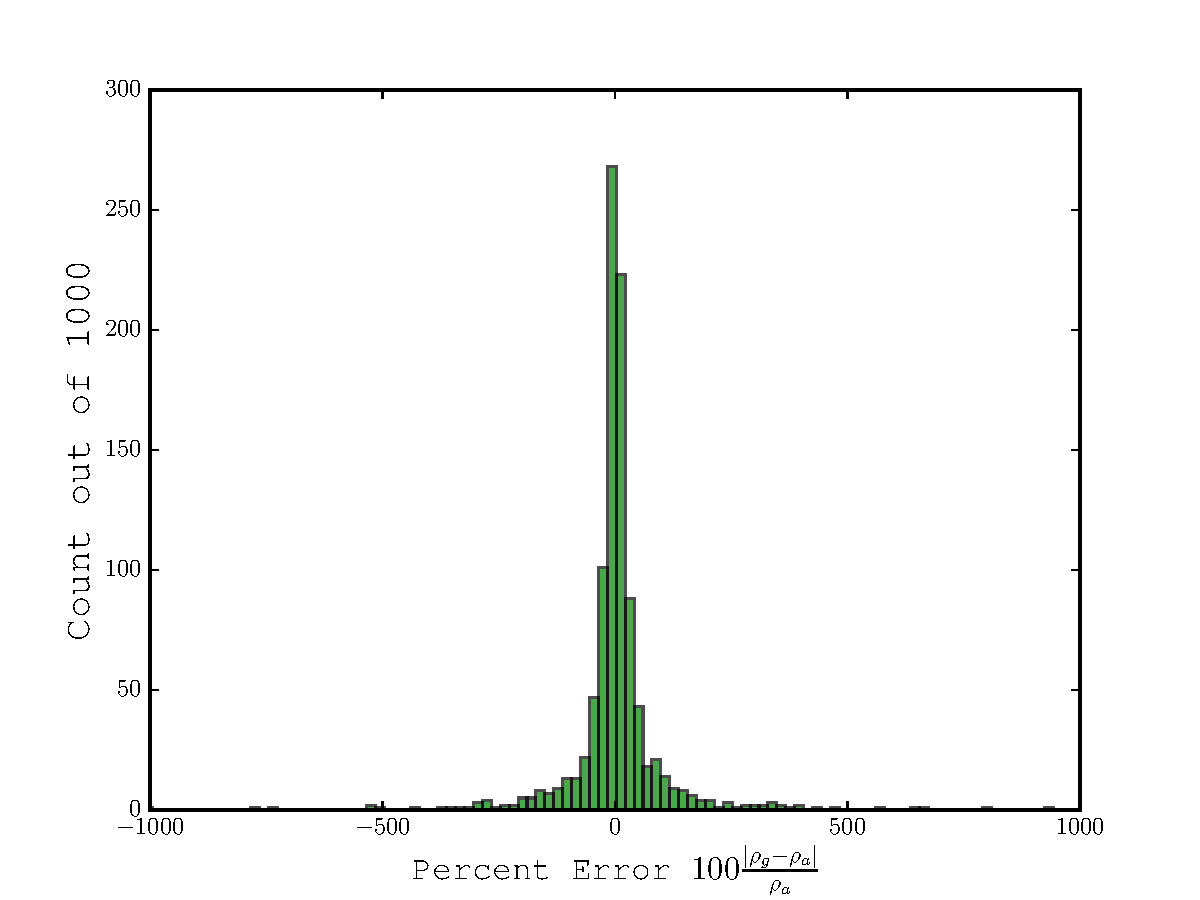
\includegraphics[width=0.77\columnwidth]{Problem2/P2.pdf}
        \vspace{-5mm}
        \caption{Histogram plot showing error $\rho_g$ is
          the approximated guess at $\rho_3$ and $\rho_a$ is the
        actual calculated $\rho_3$.}
        \label{fig:P2}
      \end{center}
    \end{figure}
\end{homeworkProblem}

\clearpage

%--------------------------------------------------------------------------
%	PROBLEM 3
%--------------------------------------------------------------------------

\begin{homeworkProblem}
  For the following data, compute by hand or via code you write
  the Pearson and Spearman correlations and Kendall's tau.
  \begin{table}[H]%
    \begin{center}
    \begin{tabular}{c c}
      \toprule%
      $X_1$ & $X_2$ \\ \midrule
      55.01 & 82.94 \\
      54.87 & 55.02 \\
      57.17 & 85.18 \\
      36.01 & -84.27 \\
      35.88 & -106.30 \\
      36.33 & -119.65 \\
      43.49 & -112.03 \\
      41.44 & -71.69 \\
      54.43 & -3.50 \\
      36.47 & 140.57 \\ \bottomrule
    \end{tabular}
    \end{center}
  \end{table}
  
  \pythonscript{Problem3/Calculations}{Script for Problem}
  Code output:\\~\\
  Pearson: 0.000672597071936\\
  Spearman: 0.587878787879\\
  Kendall: 0.5111111111111111\\
\end{homeworkProblem}

\clearpage

%--------------------------------------------------------------------------
%	PROBLEM 4
%--------------------------------------------------------------------------

\begin{homeworkProblem}
  Demonstrate the tail dependence of a bivariate normal
  random variable is 0.\\~\\
  \problemAnswer{
    The bivariate Gaussian copula is defined as:
    \begin{equation*}
      C_N(u,v)=\Phi_\rho(\Phi^{-1}(u),\Phi^{-1}(v))
    \end{equation*}
    Where:
    \begin{align*}
      \Phi^{-1}(q)&=\mu+\sigma\sqrt{2}erf^{-1}(2q-1)
    \end{align*}
    Evaluated at $q=0$:
    \begin{equation*}
      \Phi^{-1}(0)=-\infty
    \end{equation*}
    Also where:
    \begin{equation*}
      \Phi_\rho(x,y)=\int_{-\infty}^{x}dx'\int_{-\infty}^{y}dy'
      \frac{1}{2\pi \sigma_x\sigma_y\sqrt{1-\rho^2}}
      exp\left[-\frac{z}{2(1-\rho^2)}\right]
    \end{equation*}
    with
    \begin{equation*}
      z=\frac{(x'-\mu_x)^2}{\sigma_x^2}-
      \frac{2\rho(x'-\mu_x)(y'-\mu_y)}{\sigma_x\sigma_y}+
      \frac{(y'-\mu_y)^2}{\sigma_y^2}
    \end{equation*}
    and
    \begin{equation*}
      \rho=\frac{E[XY]-E[X]E[Y]}{\sigma_x\sigma_y}
    \end{equation*}
    \textbf{Note: McClarren is a poo poo head}
    \begin{align*}
      \Phi_\rho(x,y)=\int_{-\infty}^{x}dx'\int_{-\infty}^{y}dy'
      \frac{1}{2\pi \sigma_x\sigma_y\sqrt{1-\rho^2}}
      exp\left[-\frac{z}{2(1-\rho^2)}\right]
    \end{align*}
  }
  \problemAnswer{
    \textbf{Tail Dependance:}\\~\\
    \begin{equation*}
      \lambda_l=\lim_{q \to 0} \frac{C(q,q)}{q}
    \end{equation*}
  }

\end{homeworkProblem}

\clearpage


%--------------------------------------------------------------------------
%	PROBLEM 5
%--------------------------------------------------------------------------

\begin{homeworkProblem}
  Another Archimedean copula is the Joe copula with generator
  \begin{equation*}
    \phi_J(t)=-log(1-(1-t)^{\theta}),
  \end{equation*}
  and
  \begin{equation*}
    \phi_{J}^{-1}=1-(1-exp(-t))^{1/\theta}.
  \end{equation*}
\end{homeworkProblem}


\clearpage


%--------------------------------------------------------------------------
%% This is an example citation \cite{Tatro2013}.
%% \bibliography{references} 
%% \bibliographystyle{plain} 

\end{document}
